\chapter{Evaluation}
\label{evaluation}

This chapter evaluates the performance of the implementation described in chapter \ref{implementation}.
Two measurements were taken to assess the performance:

\begin{itemize}
    \item The time required to process the ready half of the receive buffer (see subsection
          \ref{implementation/software/packet-processing-task}). This measurement will be called
          \textbf{time per buffer} in the following.
    \item The time that passes between two calls of \lstinline{process_buffer} function (again, see
          subsection \ref{implementation/software/packet-processing-task}). This measurement will be
          called \textbf{time between buffers} in the following.
\end{itemize}

The \textit{time per buffer} measures the performance of the part of the system that actually deals
with incoming data. It does not measure idle time and synchronization overhead. The
\textit{time between buffers} on the other hand measures the performance of the entire system. It
indicates how much time passes between two opportunities to process incoming data. This means that
if this time does not exceed the maximum amount of time of \SI{16}{\milli\second} calculated in
subsection \ref{implementation/software/packet-processing-task}, no incoming data will be lost.

In addition, the perceived responsiveness of the UI is also reported. These observations are entirely
subjective and only meant to give an impression of the responsiveness to be expected.

The source code of the firmware and scripts used for measurements as well as the results can be found
at \url{https://github.com/Laegluin/embedded_debug_interface_for_robots/tree/thesis-benchmark-ref}.
The version used for measurements is tagged as \lstinline{thesis-benchmark-ref}.

All code was compiled with GCC 6.3.1 with maximum optimizations, link-time optimization and no
exception support (\lstinline{-O3 -flto -fno-exceptions}).

Section \ref{evaluation/measurement-method} describes the method used to obtain the measurements and
section \ref{evaluation/results} presents the results.

\section{Measurement Method}
\label{evaluation/measurement-method}

The FT232R USB to UART converter listed in section \ref{implementation/hardware} was used to simulate
an actual \textit{RS-485} bus. Three different kinds of simulated traffic were used:

\begin{itemize}
    \item A trace of real traffic from the bus of a robot of the \textit{Hamburg Bit-Bots}.
    \item Synthetic traffic of 20 devices consisting of \textit{Ping} instructions followed by
          \textit{Read}, \textit{Write}, \textit{Sync Read}, \textit{Sync Write}, \textit{Bulk Read}
          and \textit{Bulk Write} instructions for each device, repeated 300 times.
    \item Synthetic traffic of 20 devices that are constantly responding to \textit{Ping} instructions.
          Devices change their model number after each \textit{Ping} instruction.
\end{itemize}

The simulated traffic was sent to the USB to UART converter in two ways:

\begin{itemize}
    \item the entire file of simulated traffic at once
    \item one packet at a time, with \SI{100}{\micro\second} delay per packet
\end{itemize}

A python script was used to send the simulated traffic. Output buffering was disabled. To minimize
the system call overhead when not adding any delay, the files containing the simulated traffic all
had a size of at least \SI{400}{KiB}. When the file was smaller, it was made bigger by simply
repeating the contents.

All combinations of the aforementioned parameters (for a total of six different combinations) were
tested as separate experiments. Before starting the experiments, the microcontroller was reset and
every view of the UI was opened at least once to ensure that every view would be updated. Measurements
were taken for at least \SI{80}{\second} after reset.

The firmware had to be modified slightly to allow for collection of the measurements. An additional
timer was used to generate an interrupt every \SI{0.1}{\milli\second}. The interrupt handler incremented
a counter every time it was called. This counter was used in calls to \lstinline{process_buffer} to
determine the current time. Thus, every measurement has an accuracy of \SI{0.1}{\milli\second}.

Measurements were stored on external RAM. After enough measurements had been taken, the microcontroller
was halted using the debugger. The debugger was then used to dump the memory that stored the
measurements. The raw data was converted to a JSON file and then plotted using two python scripts.

The interrupts generated by the additional timer and the extra code to store the measurements on
comparatively slow external RAM imposed overhead that is not present during normal execution. As a
consequence, all times measured are an upper bound on the expected values. The differences should be
minimal, however.

\section{Results}
\label{evaluation/results}

This section presents the results of the experiments for each of the six combinations mentioned
above. Every experiment is presented in a separate subsection. There are four different plots
for each experiment. The scatter plots show the \textit{time per buffer} and
\textit{time between buffers} over time. Since each data point represents a duration, points in the
plots are placed at the geometric mean of the start and end point of the duration. The histograms
show the distribution of durations for each scatter plot.

Subsection \ref{evaluation/results/results-by-experiment} contains tables for maximum, median, mean
and minimum \textit{time per buffer} and \textit{time between buffers} for each experiment. It also
shows the data rates that can be derived from the results in an additional table.

The first \SI{20}{\second} of measurements were discarded to allow for the manual setup, the next
\SI{60}{\second} were used to generate the following plots and tables.

\clearpage
\subsection{Trace, no delay}
\label{evaluation/results/trace-no-delay}

\begin{figure}[H]
    \makebox[\textwidth][c]{
        \begin{subfigure}[t]{0.61\textwidth}
            \centering
            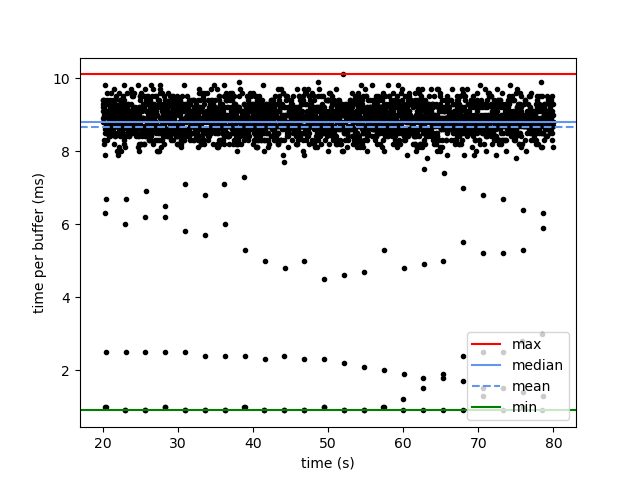
\includegraphics[scale=0.55]{img/trace_no_wait_per_buffer_scatter.png}
            \caption{Scatter plot of \textit{time per buffer}}
        \end{subfigure}%
        \begin{subfigure}[t]{0.61\textwidth}
            \centering
            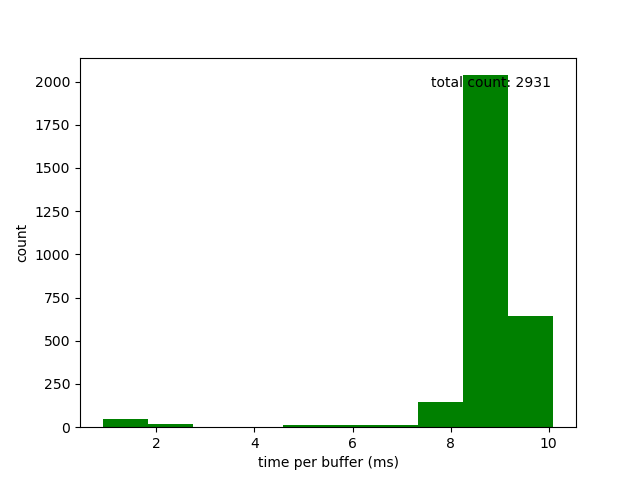
\includegraphics[scale=0.55]{img/trace_no_wait_per_buffer_hist.png}
            \caption{Histogram of \textit{time per buffer}}
        \end{subfigure}
    }

    \makebox[\textwidth][c]{
        \begin{subfigure}[t]{0.61\textwidth}
            \centering
            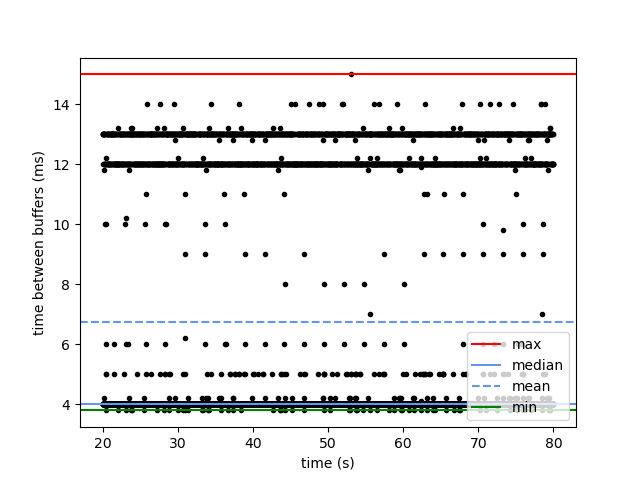
\includegraphics[scale=0.55]{img/trace_no_wait_between_buffers_scatter.png}
            \caption{Scatter plot of \textit{time between buffers}}
        \end{subfigure}%
        \begin{subfigure}[t]{0.61\textwidth}
            \centering
            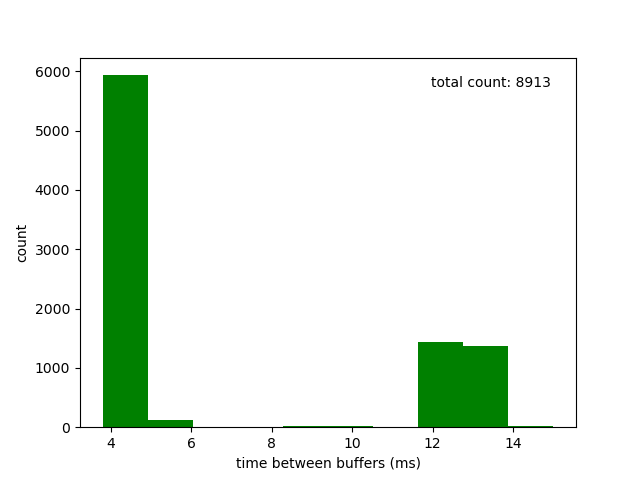
\includegraphics[scale=0.55]{img/trace_no_wait_between_buffers_hist.png}
            \caption{Histogram of \textit{time between buffers}}
        \end{subfigure}
    }

    \caption{\textit{Time per buffer} and \textit{time between buffers} for trace traffic with no delay}
    \label{evaluation/results/trace-no-delay/plots}
\end{figure}

\paragraph{UI responsiveness}

The UI was responsive, there was regular but short stuttering.
\bigbreak

Most of the measurements of \textit{time per buffer} are clustered around \SIrange{8}{10}{\milli\second}.
There are noticeable exceptions that occur at regular intervals. These are most likely packets that
were not transmitted correctly at the time the trace was recorded. Because they were malformed, they
were ignored after parsing, leading to less time spent processing the buffer that contained these
errors. Transmission errors that occurred during the measurements are unlikely to have had a significant
impact due to the extremely short cable length. In addition, these errors would not appear at regular
intervals, while recorded errors would be repeated every time the trace is repeated, which happened
frequently since the size of the trace was only \SI{516}{KiB}.

There are two distincts spikes in the \textit{time between buffers}. The higher spike is caused by
those measurements that were taken while a buffer was being processed. Most of the measurements a
around \SI{4}{\milli\second}. These are the measurements taken when there was no data to process.
They are the majority, indicating that higher data rates could be handled without a problem.

It is unclear why the \textit{time between buffers} is so tightly clustered around certain times.
It is possible that these clusters were caused by synchronization with one of the mutexes. Since the
time the UI task was holding a lock was always the same and since FreeRTOS could only preempt a task
every millisecond, there was only a very limited set of possible wait times for the packet processing
task. These wait times may have been what caused the tight clustering.

\clearpage
\subsection{Trace, \SI{100}{\micro\second} delay}
\label{evaluation/results/trace-100us-delay}

\begin{figure}[H]
    \makebox[\textwidth][c]{
        \begin{subfigure}[t]{0.61\textwidth}
            \centering
            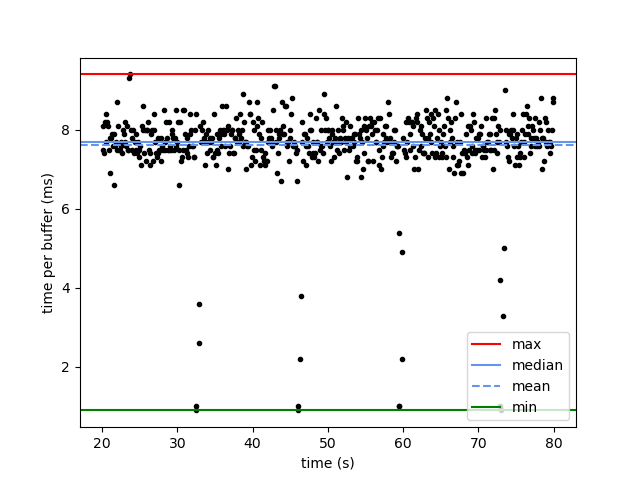
\includegraphics[scale=0.55]{img/trace_wait_100us_per_buffer_scatter.png}
            \caption{Scatter plot of \textit{time per buffer}}
        \end{subfigure}%
        \begin{subfigure}[t]{0.61\textwidth}
            \centering
            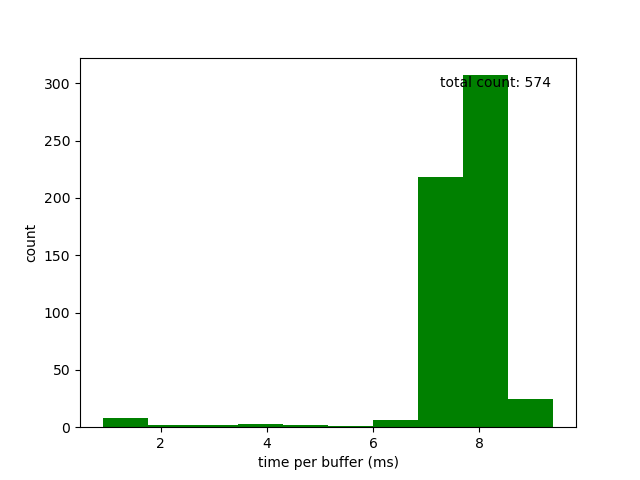
\includegraphics[scale=0.55]{img/trace_wait_100us_per_buffer_hist.png}
            \caption{Histogram of \textit{time per buffer}}
        \end{subfigure}
    }

    \makebox[\textwidth][c]{
        \begin{subfigure}[t]{0.61\textwidth}
            \centering
            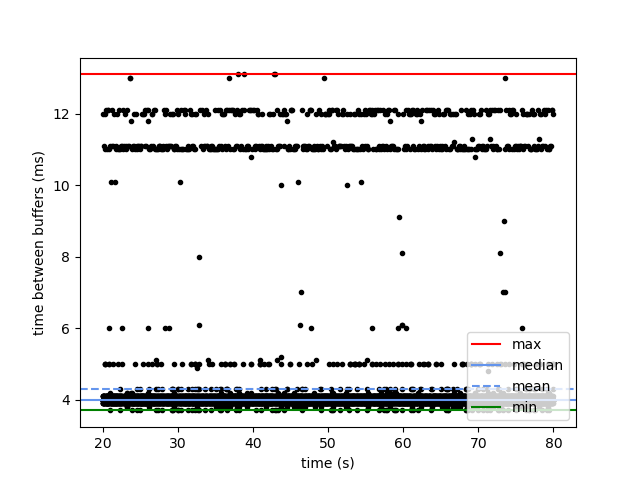
\includegraphics[scale=0.55]{img/trace_wait_100us_between_buffers_scatter.png}
            \caption{Scatter plot of \textit{time between buffers}}
        \end{subfigure}%
        \begin{subfigure}[t]{0.61\textwidth}
            \centering
            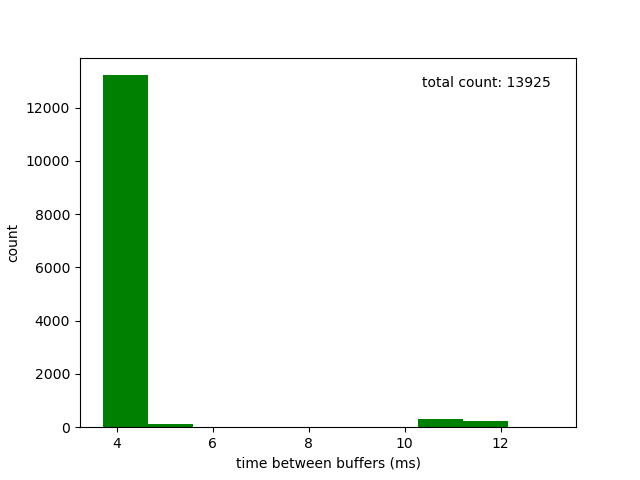
\includegraphics[scale=0.55]{img/trace_wait_100us_between_buffers_hist.png}
            \caption{Histogram of \textit{time between buffers}}
        \end{subfigure}
    }

    \caption{\textit{Time per buffer} and \textit{time between buffers} for trace traffic with \SI{100}{\micro\second} delay}
    \label{evaluation/results/trace-100us-delay/plots}
\end{figure}

\paragraph{UI responsiveness}

The UI was responsive, there was only occasional minimal stuttering.
\bigbreak

All measurements look extremely similar to those in the experiment with no delay. Since the additional
delay reduced the effective data rate (see table \ref{evaluation/results/results-by-experiment/data-rates}),
there were less packets processed in the same time frame and the influence of malformed packets was
not as severe.

The \textit{time between buffers} is absolutely dominated by measurements taken when there was no
data to process. This is not suprising, as even less time was spent processing data when there was
also a delay per packet.

\clearpage
\subsection{Synthetic Read/Write instructions, no delay}
\label{evaluation/results/synthetic-read-write-instructions-no-delay}

\begin{figure}[H]
    \makebox[\textwidth][c]{
        \begin{subfigure}[t]{0.61\textwidth}
            \centering
            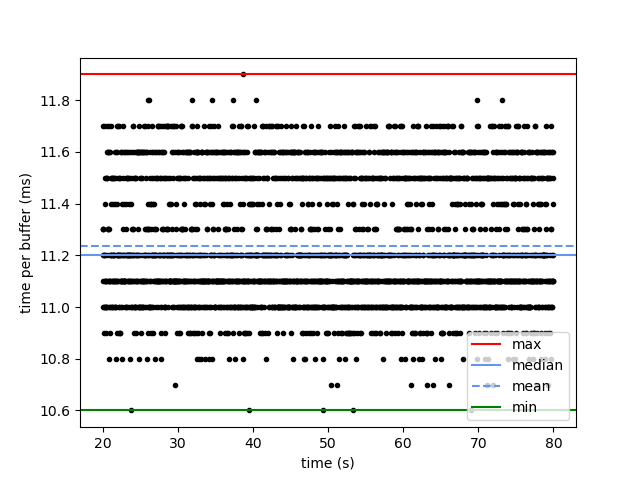
\includegraphics[scale=0.55]{img/synthetic_read_writes_no_wait_per_buffer_scatter.png}
            \caption{Scatter plot of \textit{time per buffer}}
        \end{subfigure}%
        \begin{subfigure}[t]{0.61\textwidth}
            \centering
            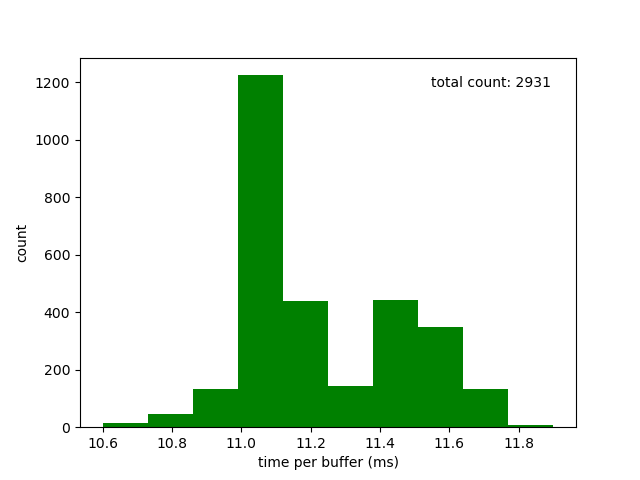
\includegraphics[scale=0.55]{img/synthetic_read_writes_no_wait_per_buffer_hist.png}
            \caption{Histogram of \textit{time per buffer}}
        \end{subfigure}
    }

    \makebox[\textwidth][c]{
        \begin{subfigure}[t]{0.61\textwidth}
            \centering
            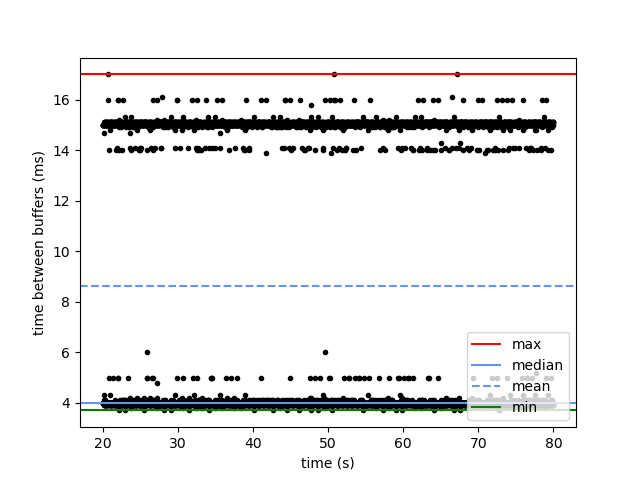
\includegraphics[scale=0.55]{img/synthetic_read_writes_no_wait_between_buffers_scatter.png}
            \caption{Scatter plot of \textit{time between buffers}}
        \end{subfigure}%
        \begin{subfigure}[t]{0.61\textwidth}
            \centering
            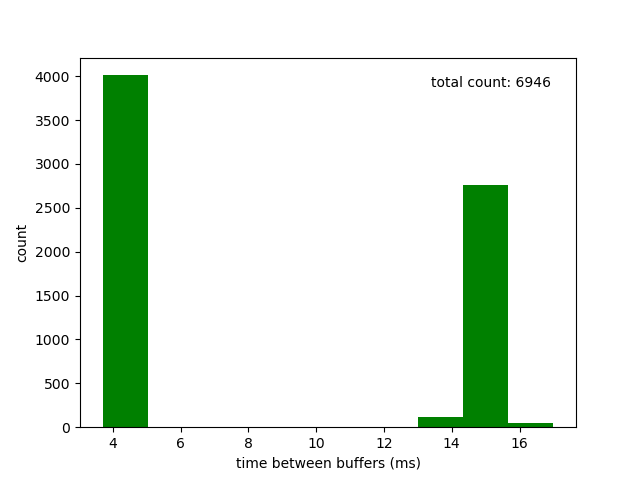
\includegraphics[scale=0.55]{img/synthetic_read_writes_no_wait_between_buffers_hist.png}
            \caption{Histogram of \textit{time between buffers}}
        \end{subfigure}
    }

    \caption{\textit{Time per buffer} and \textit{time between buffers} for synthetic read/write traffic with no delay}
    \label{evaluation/results/synthetic-read-write-instructions-no-delay/plots}
\end{figure}

\paragraph{UI responsiveness}

The UI was still usable but there was heavy stuttering. Using the UI was not pleasant.
\bigbreak

Compared to the experiments using the recorded trace, there are almost no outliers in the measurements.
The synthetic nature of the data is clearly visible. Measurements are extremely clustered and all
clusters are very close to each other.

These clusters were most likely caused by the different types of packets that are part of the data.
The same types of packets were always sent as a sequence. Every type had a slightly different length
and took a slightly different path through the program. This did not make a significant difference to
the overall time but it was enough to consistently change the time it took to process a buffer,
depending on the types of packets it contained.

\clearpage
\subsection{Synthetic Read/Write instructions, \SI{100}{\micro\second} delay}
\label{evaluation/results/synthetic-read-write-instructions-100us-delay}

\begin{figure}[H]
    \makebox[\textwidth][c]{
        \begin{subfigure}[t]{0.61\textwidth}
            \centering
            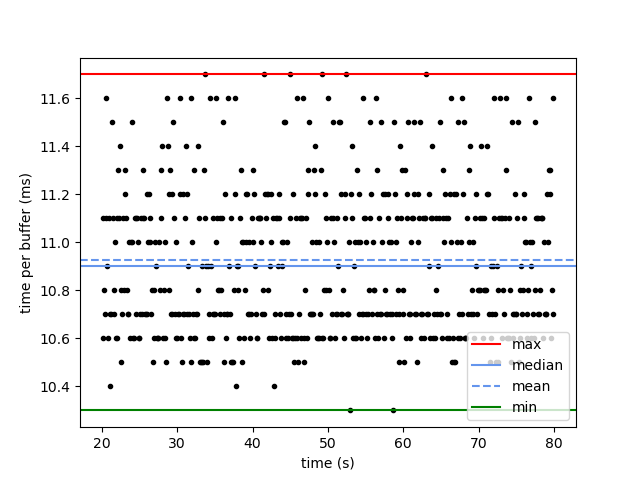
\includegraphics[scale=0.55]{img/synthetic_read_writes_wait_100us_per_buffer_scatter.png}
            \caption{Scatter plot of \textit{time per buffer}}
        \end{subfigure}%
        \begin{subfigure}[t]{0.61\textwidth}
            \centering
            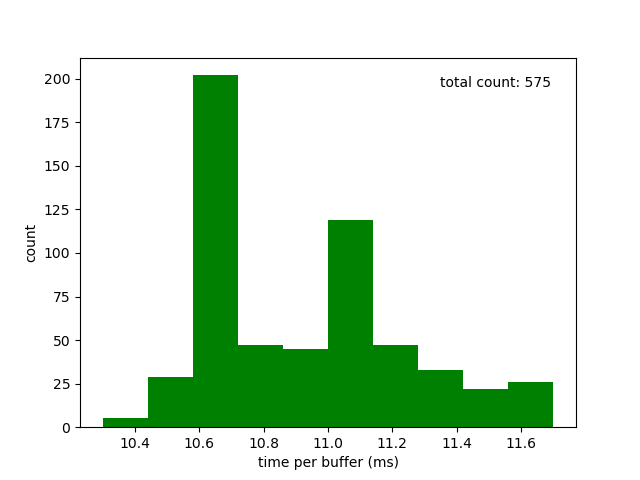
\includegraphics[scale=0.55]{img/synthetic_read_writes_wait_100us_per_buffer_hist.png}
            \caption{Histogram of \textit{time per buffer}}
        \end{subfigure}
    }

    \makebox[\textwidth][c]{
        \begin{subfigure}[t]{0.61\textwidth}
            \centering
            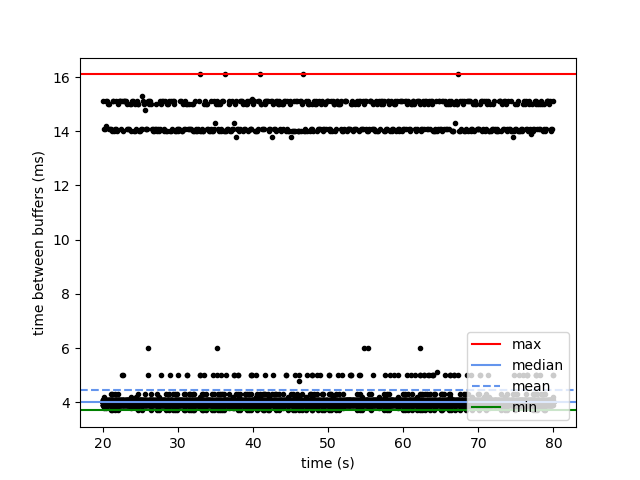
\includegraphics[scale=0.55]{img/synthetic_read_writes_wait_100us_between_buffers_scatter.png}
            \caption{Scatter plot of \textit{time between buffers}}
        \end{subfigure}%
        \begin{subfigure}[t]{0.61\textwidth}
            \centering
            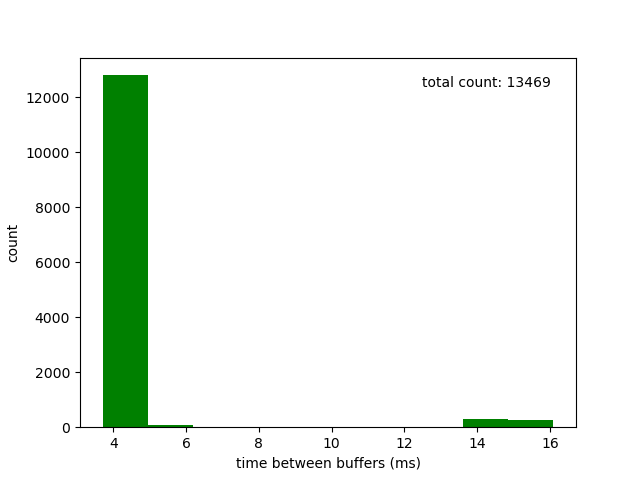
\includegraphics[scale=0.55]{img/synthetic_read_writes_wait_100us_between_buffers_hist.png}
            \caption{Histogram of \textit{time between buffers}}
        \end{subfigure}
    }

    \caption{\textit{Time per buffer} and \textit{time between buffers} for synthetic read/write traffic with \SI{100}{\micro\second} delay}
    \label{evaluation/results/synthetic-read-write-instructions-100us-delay/plots}
\end{figure}

\paragraph{UI responsiveness}

The UI was responsive, there was only occasional short stuttering.
\bigbreak

Like the experiment using the recorded trace, results when adding a delay per packet are very similar
to those without delay. Again, clusters in the \textit{time per buffer} plots are less pronounced as
there are less measurements and the measurements for the \textit{time between buffers} are dominated
by constant overhead.

\clearpage
\subsection{Synthetic Ping instructions, no delay}
\label{evaluation/results/synthetic-ping-instructions-no-delay}

\begin{figure}[H]
    \makebox[\textwidth][c]{
        \begin{subfigure}[t]{0.61\textwidth}
            \centering
            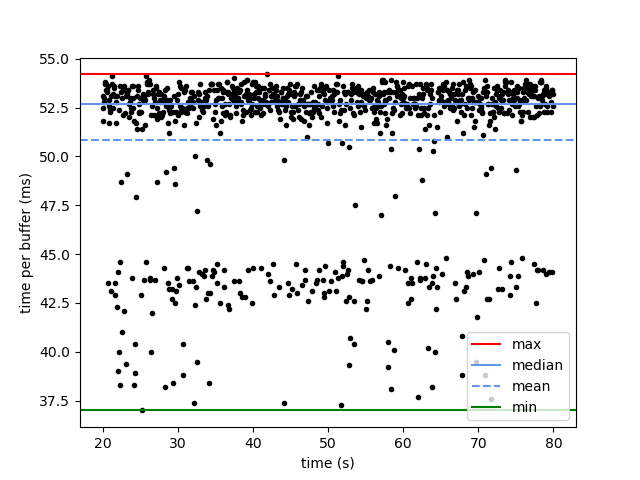
\includegraphics[scale=0.55]{img/synthetic_pings_no_wait_per_buffer_scatter.png}
            \caption{Scatter plot of \textit{time per buffer}}
        \end{subfigure}%
        \begin{subfigure}[t]{0.61\textwidth}
            \centering
            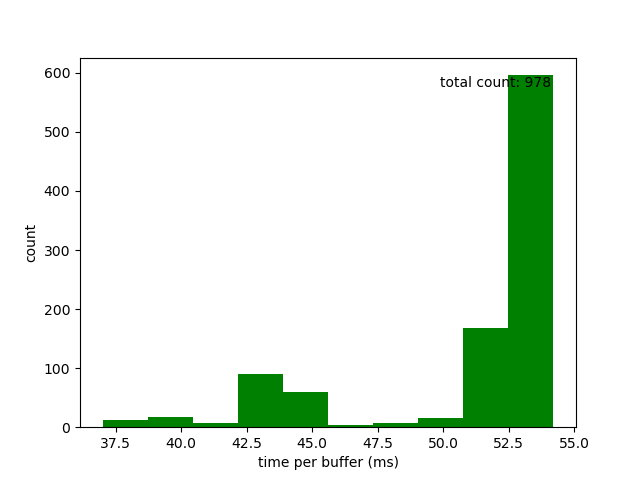
\includegraphics[scale=0.55]{img/synthetic_pings_no_wait_per_buffer_hist.png}
            \caption{Histogram of \textit{time per buffer}}
        \end{subfigure}
    }

    \makebox[\textwidth][c]{
        \begin{subfigure}[t]{0.61\textwidth}
            \centering
            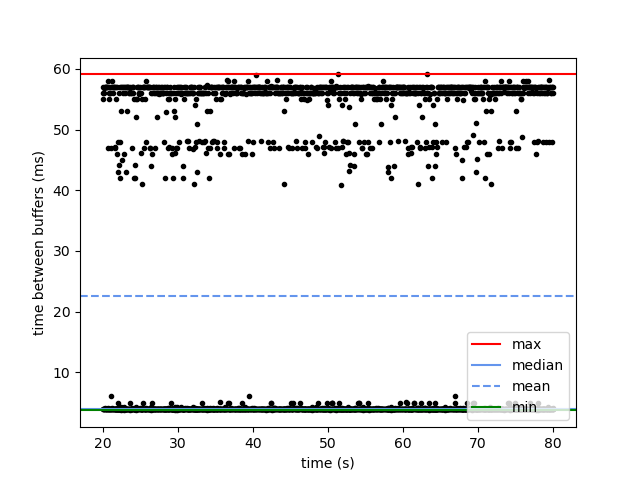
\includegraphics[scale=0.55]{img/synthetic_pings_no_wait_between_buffers_scatter.png}
            \caption{Scatter plot of \textit{time between buffers}}
        \end{subfigure}%
        \begin{subfigure}[t]{0.61\textwidth}
            \centering
            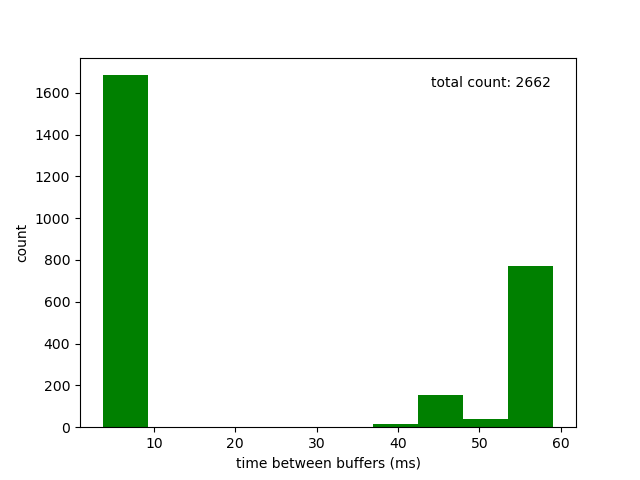
\includegraphics[scale=0.55]{img/synthetic_pings_no_wait_between_buffers_hist.png}
            \caption{Histogram of \textit{time between buffers}}
        \end{subfigure}
    }

    \caption{\textit{Time per buffer} and \textit{time between buffers} for synthetic ping traffic with no delay}
    \label{evaluation/results/synthetic-ping-instructions-no-delay/plots}
\end{figure}

\paragraph{UI responsiveness}

The UI was not responsive at all. While it was still possible to use, scrolling did not work properly
and any action caused significant and noticeable delays.
\bigbreak

The results for the \textit{time per buffer} are significantly worse than in the previous experiments.
The maximum \textit{time per buffer} exceeds \SI{50}{\milli\second} and there are many outliers.
These outliers were most likely caused by errors during parsing: since the buffers were not processed
quickly enough, the DMA controller was overwriting buffers as they were being read.

The \textit{time between buffers} reflects the measurements for \textit{time per buffer}. However,
it is notable that there are many measurements of only about \SI{4}{\milli\second}, even though the
processing was too slow. This is because after processing one buffer, there was a high likelyhood
that the next buffer was not currently ready. Data was not lost during these waits but during
processing itself, meaning that the amount of waits only decreased because more time was spent
processing data.

Because so much time was spent processing data, the amount of time dedicated to the UI decreased and
the latency increased. The high latencies caused problems with input handling since it could not be
processed in time. Less time for the UI task also meant the real time required for rendering the UI
increased.

\clearpage
\subsection{Synthetic Ping instructions, \SI{100}{\micro\second} delay}
\label{evaluation/results/synthetic-ping-instructions-100us-delay}

\begin{figure}[H]
    \makebox[\textwidth][c]{
        \begin{subfigure}[t]{0.61\textwidth}
            \centering
            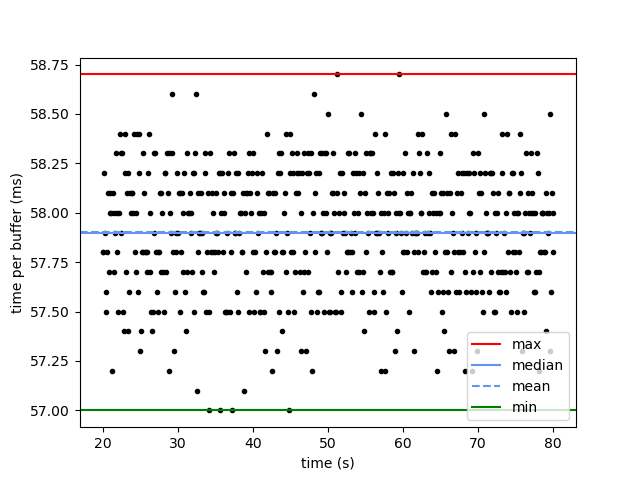
\includegraphics[scale=0.55]{img/synthetic_pings_wait_100us_per_buffer_scatter.png}
            \caption{Scatter plot of \textit{time per buffer}}
        \end{subfigure}%
        \begin{subfigure}[t]{0.61\textwidth}
            \centering
            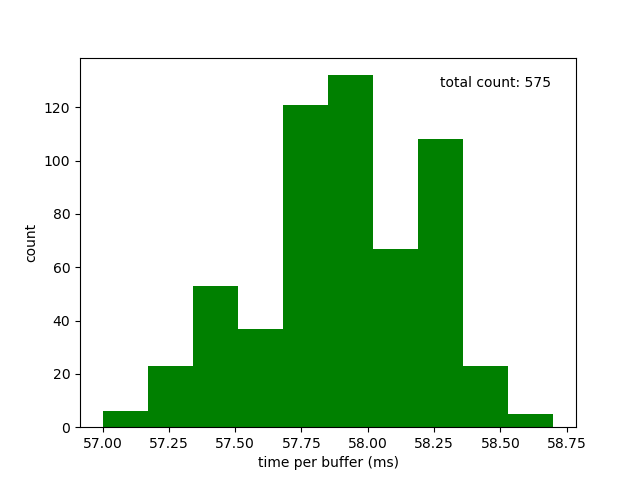
\includegraphics[scale=0.55]{img/synthetic_pings_wait_100us_per_buffer_hist.png}
            \caption{Histogram of \textit{time per buffer}}
        \end{subfigure}
    }

    \makebox[\textwidth][c]{
        \begin{subfigure}[t]{0.61\textwidth}
            \centering
            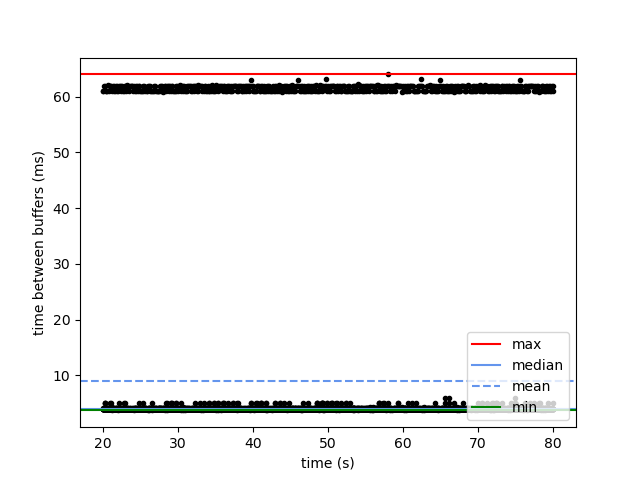
\includegraphics[scale=0.55]{img/synthetic_pings_wait_100us_between_buffers_scatter.png}
            \caption{Scatter plot of \textit{time between buffers}}
        \end{subfigure}%
        \begin{subfigure}[t]{0.61\textwidth}
            \centering
            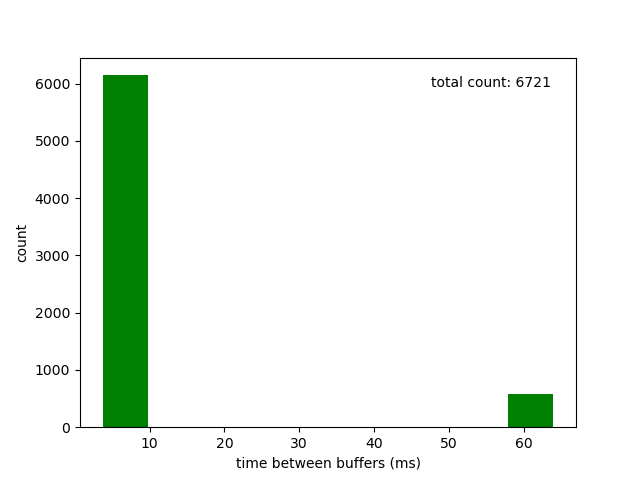
\includegraphics[scale=0.55]{img/synthetic_pings_wait_100us_between_buffers_hist.png}
            \caption{Histogram of \textit{time between buffers}}
        \end{subfigure}
    }

    \caption{\textit{Time per buffer} and \textit{time between buffers} for synthetic ping traffic with \SI{100}{\micro\second} delay}
    \label{evaluation/results/synthetic-ping-instructions-100us-delay/plots}
\end{figure}

\paragraph{UI responsiveness}

The UI was mostly usable but there was significant stuttering. Scrolling mostly worked but was not
pleasant to use. The were noticeable but not significant delays when interacting with buttons. 
\bigbreak

Results with delay per packet look remarkably similar to those for the experiments with synthetic
\textit{Read} and \textit{Write} instructions. The only difference is that all times increased
drastically to about \SIrange{57}{59}{\milli\second}. The reason is that while the average
\textit{time per buffer} was still about four times higher than the allowed maximum of
\SI{16}{\milli\second}, the delay per packet slowed down the effective data rate enough to make the
actual allowed maximum greater than the measured maximum \textit{time per buffer}.

This can clearly be seen when comparing the effective data rates in table \ref{evaluation/results/results-by-experiment/data-rates}:
the effective data rates with added delay are all comparable, whereas the effective data rate for
synthetic \textit{Ping} instructions with no delay is significantly lower than the others.

It is also the reason the UI was so much more responsive than without any delay. The problems caused
by high latencies were still present but the UI task did have enough time to render the UI at a
sufficient speed.

\clearpage
\subsection{Results by Experiment}
\label{evaluation/results/results-by-experiment}

\begin{table}[h]
    \centering
    \renewcommand{\arraystretch}{1.1}
    \begin{tabularx}{\textwidth}{|>{\raggedleft\arraybackslash}X||c|c|c|c|}
        \hline
        \textbf{Experiment} & \textbf{Maximum} & \textbf{Median} & \textbf{Mean} & \textbf{Minimum} \\
        \hline
        
        \nameref{evaluation/results/trace-no-delay} &
        \SI{10.1}{\milli\second} &
        \SI{8.8}{\milli\second} &
        \SI{8.6}{\milli\second} &
        \SI{0.9}{\milli\second}
        \\
        \hline

        \nameref{evaluation/results/trace-100us-delay} &
        \SI{9.4}{\milli\second} &
        \SI{7.7}{\milli\second} &
        \SI{7.6}{\milli\second} &
        \SI{0.9}{\milli\second}
        \\
        \hline

        \nameref{evaluation/results/synthetic-read-write-instructions-no-delay} &
        \SI{11.9}{\milli\second} &
        \SI{11.2}{\milli\second} &
        \SI{11.2}{\milli\second} &
        \SI{10.6}{\milli\second}
        \\
        \hline

        \nameref{evaluation/results/synthetic-read-write-instructions-100us-delay} &
        \SI{11.7}{\milli\second} &
        \SI{10.9}{\milli\second} &
        \SI{10.9}{\milli\second} &
        \SI{10.3}{\milli\second}
        \\
        \hline

        \nameref{evaluation/results/synthetic-ping-instructions-no-delay} &
        \SI{54.2}{\milli\second} &
        \SI{52.7}{\milli\second} &
        \SI{50.8}{\milli\second} &
        \SI{37.0}{\milli\second}
        \\
        \hline

        \nameref{evaluation/results/synthetic-ping-instructions-100us-delay} &
        \SI{58.7}{\milli\second} &
        \SI{57.9}{\milli\second} &
        \SI{57.9}{\milli\second} &
        \SI{57.0}{\milli\second}
        \\
        \hline
    \end{tabularx}
    \caption{Maximum, median, mean and minimum \textit{time per buffer} for each experiment}
\end{table}

\begin{table}[h]
    \centering
    \renewcommand{\arraystretch}{1.1}
    \begin{tabularx}{\textwidth}{|>{\raggedleft\arraybackslash}X||c|c|c|c|}
        \hline
        \textbf{Experiment} & \textbf{Maximum} & \textbf{Median} & \textbf{Mean} & \textbf{Minimum} \\
        \hline

        \nameref{evaluation/results/trace-no-delay} &
        \SI{15.0}{\milli\second} &
        \SI{4.0}{\milli\second} &
        \SI{6.7}{\milli\second} &
        \SI{3.8}{\milli\second}
        \\
        \hline

        \nameref{evaluation/results/trace-100us-delay} &
        \SI{13.1}{\milli\second} &
        \SI{4.0}{\milli\second} &
        \SI{4.3}{\milli\second} &
        \SI{3.7}{\milli\second}
        \\
        \hline

        \nameref{evaluation/results/synthetic-read-write-instructions-no-delay} &
        \SI{17.0}{\milli\second} &
        \SI{4.0}{\milli\second} &
        \SI{8.6}{\milli\second} &
        \SI{3.7}{\milli\second}
        \\
        \hline

        \nameref{evaluation/results/synthetic-read-write-instructions-100us-delay} &
        \SI{16.1}{\milli\second} &
        \SI{4.0}{\milli\second} &
        \SI{4.5}{\milli\second} &
        \SI{3.7}{\milli\second}
        \\
        \hline

        \nameref{evaluation/results/synthetic-ping-instructions-no-delay} &
        \SI{59.1}{\milli\second} &
        \SI{4.0}{\milli\second} &
        \SI{22.6}{\milli\second} &
        \SI{3.7}{\milli\second}
        \\
        \hline

        \nameref{evaluation/results/synthetic-ping-instructions-100us-delay} &
        \SI{64.0}{\milli\second} &
        \SI{4.0}{\milli\second} &
        \SI{8.9}{\milli\second} &
        \SI{3.7}{\milli\second}
        \\
        \hline
    \end{tabularx}
    \caption{Maximum, median, mean and minimum \textit{time between buffers} for each experiment}
\end{table}

\clearpage
\begin{table}[ht]
    \centering
    \renewcommand{\arraystretch}{1.1}
    \begin{tabularx}{\textwidth}{|>{\raggedleft\arraybackslash}X||c|c|c|c|}
        \hline
        \textbf{Experiment} & \textbf{Effective data rate} & \textbf{Processing data rate} \\
        \hline

        \nameref{evaluation/results/trace-no-delay} &
        \SI{1600717}{bit\per\second} &
        \SI{3788589}{bit\per\second}
        \\
        \hline

        \nameref{evaluation/results/trace-100us-delay} &
        \SI{313481}{bit\per\second} &
        \SI{4306544}{bit\per\second}
        \\
        \hline

        \nameref{evaluation/results/synthetic-read-write-instructions-no-delay} &
        \SI{1600717}{bit\per\second} &
        \SI{2916174}{bit\per\second}
        \\
        \hline

        \nameref{evaluation/results/synthetic-read-write-instructions-100us-delay} &
        \SI{314027}{bit\per\second} &
        \SI{2999109}{bit\per\second}
        \\
        \hline

        \nameref{evaluation/results/synthetic-ping-instructions-no-delay} &
        \SI{534118}{bit\per\second} &
        \SI{644432}{bit\per\second}
        \\
        \hline

        \nameref{evaluation/results/synthetic-ping-instructions-100us-delay} &
        \SI{314027}{bit\per\second} &
        \SI{565894}{bit\per\second}
        \\
        \hline
    \end{tabularx}
    \caption{
        The effective and processing data rates for each experiment. The effective data rate is the
        number of bits that were received divided by the duration of the experiment (\SI{60}{\second}).
        The processing data rate is the rate at which the actual packet processing task could in
        theory process packets. It is calculated by dividing the number of bits that were received
        by the time spent processing them (the sum of all \textit{time per buffer} measurements).
    }
    \label{evaluation/results/results-by-experiment/data-rates}
\end{table}
